% !TeX root = orbits.tex
% !TeX Program=pdfLaTeX

\part{Fun with ellipses}

%%%%%%%%%%%%%%%%%%%%%%%%%%%%%%%%%%%%%%%%%%%%%%%%%%%%%%%%%%%%%

\chapter{Constructing an ellipse}\label{s.constructing}

There are many methods and tools for drawing ellipses. The simplest method is the \emph{gardener's method} (Figure~\ref{f.gardener}): given $a$, the length of the semi-major axis and two points $S,H$, the foci, attach a rope of length $2a$ to two stakes at the foci and pull taut with a pencil. As the pencil moves around the foci maintaining tension on the rope, it will trace an ellipse.

%%%%%%%%%%%%%%%%%%%%%%%%%%%%%%%%%%%%%%%%%%%%%%%%%%%%%%%%%%%%%

\begin{figure}[b]
\begin{center}
\begin{tikzpicture}
\clip (-3.1,-2.1) rectangle +(6.2,4.2);
% Size and center of the ellipse
\def\a{3}
\def\b{2}
\def\angle{40}
\pic{ellipse={{\a}/{\b}}};
\draw[thick,red] (O) ellipse[x radius=\a,y radius= \b];
% Locate the foci
\coordinate (F1) at ({-sqrt(\a*\a-\b*\b)},0);
\coordinate (F2) at ({sqrt(\a*\a-\b*\b)},0);
\draw[blue] (F1) circle[radius=2pt];
\draw[blue] (F2) circle[radius=2pt];
\node[below] at (F1) {$S$};
\node[below] at (F2) {$H$};

\coordinate (P) at ({\angle}:{\a} and {\b});
\draw[blue] (P) circle[radius=2pt];
\draw[blue] (F1) -- (P) -- (F2);
\node[above right] at (P) {$P$};

\end{tikzpicture}
\caption{The gardener method for drawing an ellipse}\label{f.gardener}
\end{center}
\end{figure}


This Section presents several more accurate methods for drawing ellipses. First, we review two methods to construct \emph{individual points} on an ellipse (Section~\ref{s.individual}).  Section~\ref{s.roulette} describes a \emph{roulette} called the \emph{Tusi couple}. This is followed by four methods of constructing an ellipse with a \emph{glissette}: Section~\ref{s.glissette} on the \emph{Trammel of Archimedes}, Section~\ref{s.articulated} on two articulated glissettes by Frans van Schooten, and Section~\ref{s.triangle-glissette} on a triangle glissette. The final Section~\ref{s.confocal} describes how to construct a \emph{confocal} ellipse.

%%%%%%%%%%%%%%%%%%%%%%%%%%%%%%%%%%%%%%%%%%%%%%%%%%%%%%%%%%

\section{Constructing individual points on an ellipse}\label{s.individual}

\subsubsection*{From an arbitrary point on the directrix}

Let us repeat without proof the construction for Theorem~\ref{thm.point-on-an-ellipse}. Assume that we are given $a$, the length of the semi-major axis and $c$, the distance of a focus from the center. Let $E$ be a point on the directrix and construct lines from $E$ through $A$ and $S$. The line through $S$ will make an angle $\alpha$ with $XS$. Construct a line from $S$ at the \emph{same angle} $\alpha$ from $ES$ and let its intersection with $EA$ be $P$. Then $P$ is a point on the ellipse (Figure~\ref{f.construct1}). 

%%%%%%%%%%%%%%%%%%%%%%%%%%%%%%%%%%%%%%%%%%%%%%%%%%%%%%%%%%

\begin{figure}[t]
\begin{center}
\begin{tikzpicture}[scale=1]

\clip (-.8,-2.2) rectangle +(9.5,4.5);

% Construct the directrix, the focus and the major axis
\coordinate (X) at (0,0);
\node[left] at (X) {$X$};
\draw[name path global=directrix] ($(X)+(0,2)$) -- ($(X)+(0,-2)$);
\coordinate (S) at (3,0);
\node[below] at (S) {$S$};

% Locate a vertex
\coordinate (A) at (2,0);
\node[above left] at (A) {$A$};
\coordinate (AP) at (7,0);
%\node[right] at ($(AP)+(1,0)$) {$N$};

% Find a convenient E and draw _paths_ to A and S
\path[name path=findE] (S) -- +(210:4);
\path [name intersections = {of = findE and directrix, by = {E} }];
\node[left] at (E) {$E$};
\path[name path=EA] (E) -- ($(E)!2.3!(A)$);
\path[name path=ES] (E) -- ($(E)!2.3!(S)$);

% Locate P by drawing a path with the same angle
\path[name path=SP] (S) -- +(60:3);
\path [name intersections = {of = EA and SP, by = {P} }];
\node[above] at (P) {$P$};
\draw[thick] (S) -- (P);

% Construct the perpendicular through P to the directrix
\path[name path=PK] (P) -- +(180:4.5);
\path [name intersections = {of = PK and directrix, by = {K} }];
\path[name path=PL] (K) -- ($(K)!1.8!(P)$);

% Locate L and label the segments
\path [name intersections = {of = PL and ES, by = {L} }];
\path (S) -- (P);

% Label the angles
\node[right,xshift=14pt,yshift=5pt] at (S) {$\alpha$};
\node[above right,xshift=9pt,yshift=10pt] at (S) {$\alpha$};

% Draw the colored triangles
\draw[red,thick] (E) -- (L);
\draw[blue,thick] (E) -- (P);
\draw (X) -- ($(AP)+(1,0)$);
\end{tikzpicture}
\end{center}
\caption{Constructing points on the ellipse}\label{f.construct1}
\end{figure}

%%%%%%%%%%%%%%%%%%%%%%%%%%%%%%%%%%%%%%%%%%%%%%%%%%%%%%%%%%%%%

\subsubsection*{From an arbitrary angle to the circumscribed and inscribed circles}

Recall the definition of the parametric representation given $a$ and $b$, the lengths of the semi-axes (Definition~\ref{def.parametric}): Construct two concentric circles, one of radius $a$ (dotted red) and one of radius $b$ (dashed blue) (Figure~\ref{f.parametric1}). For an arbitrary angle $t$, construct a ray that intersects the two circles at $P_O$ and $P_I$. Draw a perpendicular from $P_I$ to the $y$-axis and a perpendicular from $P_O$ to the $x$-axis. Their intersection $P$ is a point on the ellipse.

%%%%%%%%%%%%%%%%%%%%%%%%%%%%%%%%%%%%%%%%%%%%%%%%%%%%%%%%%%%%%

\begin{figure}[b]
\begin{center}
\begin{tikzpicture}
\clip (-3.1,-3.3) rectangle +(6.5,6.6);
% Size and center of the ellipse
\def\a{3}
\def\b{2}
\coordinate (C) at (0,0);
\node[below left,xshift=2pt] at (C) {$O$};

% Draw an ellipse and the inner and outer circles
\draw[name path=ellipse] (C) ellipse[x radius=\a,y radius= \b];
\draw[very thick,dotted,red,name path=outer] (C) circle[radius=\a];
\draw[thick,dashed,blue,name path=inner] (C) circle[radius=\b];

% Locate P on the ellipse
\path[name path=toP] (C) -- +(30:4);
\path [name intersections = {of = ellipse and toP, by = {P} }];

% Label the angle of CP
\node[above right,xshift=8pt,yshift=-2pt] at (C) {$t$};

% Draw major and minor axes
\draw[name path=yplus,thick] (C) -- +(0,\a);
\node[above left] at (0,\b) {$B$};
\draw[thick] (C) -- +(0,-\a);
\draw[name path=xplus] (C) -- +(\a,0) node[right] {$A$};
\draw (C) -- +(-\a,0);

% Find intersection PI of line from center to P and the inner circle
\node[below right,xshift=-3pt,yshift=-4pt] at (P) {$P$};
\vertexsm{P};
\path[name path=horiz] (P) -- +(-\a,0);
\path [name intersections = {of = inner and horiz, by = {PI} }];

% Extend ray C->PI to outer circle and label intersection PO
\path[name path=ray] (C) -- ($(C) !1.7! (PI)$);
\path [name intersections = {of = outer and ray, by = {PO} }];

% Project PO on x axis
\path[thick,name path=horizPO] (PO) -- +(0,-\a);
\path [name intersections = {of = xplus and horizPO, by = {xint} }];
\draw (PO) -- (xint);
\draw[<->,style={shorten <= 2pt},thick] ($(C)+(0,-5pt)$) --
  node[below,xshift=-4pt] {$a\cos t$} ($(xint)+(0,-5pt)$);

% Project PI on y axis
\path [name intersections = {of = yplus and horiz, by = {yint} }];
\draw[<->,thick] ($(C)+(-6pt,0)$) -- 
  node[left,xshift=1pt] {$b\sin t$} ($(yint)+(-6pt,0)$);
\draw (P) -- (yint);

% Draw blue and red lines from C to PI and PO
\draw[thick,blue] (C) -- (PI);
\draw[thick,red] (PI) -- (PO);

% Dots at vertices
\vertexsmcolor{PI}{blue};
\vertexsmcolor{PO}{red};
\node[below,yshift=-4pt] at (PI) {$P_I$};
\node[above right] at (PO) {$P_O$};
%\vertexsm{C};
%\vertexsm{P};

\end{tikzpicture}
\caption{Parametric representation of an ellipse}\label{f.parametric1}
\end{center}
\end{figure}

%%%%%%%%%%%%%%%%%%%%%%%%%%%%%%%%%%%%%%%%%%%%%%%%%%%%%%%%%%%%%%%%

\section{A roulette for drawing an ellipse---the Tusi couple}\label{s.roulette}

A \emph{roulette} is a curve generated by one curve $c_1$ \emph{rolling} on another curve $c_2$. An ellipse can be generated by a circle of radius $r$ rotating within the circumference of a circle of radius $2r$.

%%%%%%%%%%%%%%%%%%%%%%%%%%%%%%%%%%%%%%%%%%%%%%%%%%%%%%%%%%%%%%%%

\begin{figure}
\begin{center}
\begin{tikzpicture}[scale=.7]
\clip (-7.5,-1) rectangle +(15,8.5);

\def\a{7}
\def\angle{60}

\coordinate (O) at (0,0);
\coordinate (AP) at ({-\a},0);
\coordinate (A) at ({\a},0);
\draw[name path=diam] (AP) -- (A);
\draw (AP) arc[start angle=180,end angle=0,radius=\a];
\node at (130:{\a+.3}) {$c_2$};

\draw[name path=smdiam] (O) -- ({\angle}:{\a}) coordinate (E);
\coordinate (C) at +({\angle}:{\a/2});
\draw[name path=circle] (C) circle[radius={\a/2}];
\path [name intersections = {of = diam and circle, by = {dummy,Q} }];
\node at ($(C)+(135:{\a/2+.3})$) {$c_1$};

%\draw (C) -- (Q) -- (E);
\coordinate (P) at ($(C)!.6!(Q)$);

\draw (P) -- ($(O)!(P)!(A)$) coordinate (N);
\path[name path=rn] (N) -- ($(N)!4!(P)$);
\path [name intersections = {of = smdiam and rn, by = {R} }];
\draw (N) -- (R);

\path[name path=prp] (P) -- +(180:3);
\path [name intersections = {of = smdiam and prp, by = {RP} }];
\draw (P) -- (RP);

\draw[rotate=90] (Q) rectangle +(8pt,8pt);
\draw[rotate=90] (N) rectangle +(8pt,8pt);
\draw[rotate=90] (P) rectangle +(8pt,8pt);

\node[below] at (A) {$A$};
\node[below] at (O) {$O$};
\node[below] at (Q) {$Q$};
\node[left] at (C) {$C$};
\node[above right] at (E) {$E$};
\node[above left,xshift=-2pt] at (N) {$N$};
\node[right] at (P) {$P$};
\node[left] at (R) {$R$};
\node[left] at (RP) {$R'$};

\node[right,xshift=3pt] at (C) {$2\alpha$};
\node[above right,xshift=4pt] at (O) {$\alpha$};

\path (C) -- node[left] {$a$} (R);
\path (C) -- node[left] {$a$} (RP);
\path (C) -- node[below,xshift=-2pt] {$a$} (P);

\draw[thick,red] (E) -- (O) -- (Q);
\draw[thick,blue] ($(C)+(2pt,-1pt)$) -- (Q);
\draw[thick,blue] ($(C)+(2pt,-3pt)$) -- ($(E)+(3pt,-1pt)$);

\vertexsmcolor{P}{blue};

\end{tikzpicture}
\caption{Constructing an ellipse from a roulette}\label{f.roulette1}
\end{center}
\end{figure}

%%%%%%%%%%%%%%%%%%%%%%%%%%%%%%%%%%%%%%%%%%%%%%%%%%%%%%%%%%%%%%%

\begin{theorem}
Let $P$ be an arbitrary point within with circle $c_1$ of the roulette. Then as $c_1$ rotates within $c_2$, the locus of $P$ is an ellipse (Figure~\ref{f.roulette1}).
\end{theorem}

%%%%%%%%%%%%%%%%%%%%%%%%%%%%%%%%%%%%%%%%%%%%%%%%%%

\begin{figure}[b]
\begin{center}
\begin{tikzpicture}[scale=.85]
\clip (-5.5,-.5) rectangle +(11,5.6);

\def\a{5}
\coordinate (O) at (0,0);
\coordinate (AP) at ({-\a},0);
\coordinate (A) at ({\a},0);
\draw[name path=diam] (AP) -- (A);
\draw (AP) arc[start angle=180,end angle=0,radius=\a];
\foreach \angle in {5,10,...,85,95,100,...,175} {
  \coordinate (R) at +({\angle}:{3*\a/4});
  \coordinate (RP) at +({\angle}:{\a/4});
  \path[name path=rn] (R) -- ($(O)!(R)!(A)$) coordinate (N);
  \path[name path=rp] (RP) -- ($(R)!(RP)!(N)$);
  \path [name intersections = {of = rn and rp, by = {P} }];
  \fill[shift only,blue] (R) circle (1pt);
  \fill[shift only,green!80!black] (RP) circle (1pt);
  \fill[shift only,red] (P) circle (1pt);
}

\coordinate (a) at +(0:{3*\a/4});
\fill[shift only,red] (a) circle (1pt);
\coordinate (a) at +(0:{\a/4});
\fill[shift only,green!80!black] (a) circle (1pt);
\coordinate (a) at +(90:{3*\a/4});
\fill[shift only,blue] (a) circle (1pt);
\coordinate (a) at +(90:{\a/4});
\fill[shift only,red] (a) circle (1pt);
\coordinate (a) at +(180:{\a/4});
\fill[shift only,green!80!black] (a) circle (1pt);
\coordinate (a) at +(180:{3*\a/4});
\fill[shift only,red] (a) circle (1pt);

\end{tikzpicture}
\caption{The loci of $P$ (red), $R$ (blue), $R'$ (green)}\label{f.roulette2}
\end{center}
\end{figure}

%%%%%%%%%%%%%%%%%%%%%%%%%%%%%%%%%%%%%%%%%%%%%

\begin{proof}
Let $C$ be the center of $c_1$ and let $O$ be the center of $c_2$. Let $E$ be an arbitrary point on $c_2$ where it is contacted by $c_1$. The radius $OE$ of length $2r$ is a chord of $c_1$ and since it equals twice the radius of $c_1$ it is a diameter. $c_1$ will intersect $OA$ at some point $Q$ and since $OE$ is a diameter of $c_1$, $\angle EQO$ is a right angle.

$\angle ECQ=2\cdot\angle EOQ=2\alpha$ because $\angle ECQ$ is a central angle of $c_1$ subtended by $EQ$ which also subtends the inscribed angle $\angle EOQ$. Therefore the arc $\widehat{EQ}$ equals $2\alpha r$. But $\angle EOQ$ is the same angle as $EOA$ and is therefore an inscribed angle of $c_2$. It follows that the arc $\widehat{EA}$ equals $2r\alpha$ and $\widehat{EA} =\widehat{EQ}$, so as $c_1$ rotates, $Q$ is always on the diameter.

Let $P$ be an arbitrary point on $CQ$ and construct $RP\parallel EQ$ and $R'P\parallel OQ$. Let $N$ be the intersection of $RP$ with $OA$. Since $CE=CQ$ are radii of $c_1$, by $RP\parallel EQ$, $\triangle PCR\sim \triangle QCE$ so $\triangle PCR$ is isosceles and $CP=CR=a$. Similarly, $\triangle PCR'$ is isosceles and $CP=CR'=a$.

Now let $c_1$ rotate within $c_2$. Since $P$ is fixed relative to $C$ and $E$ is fixed relative to $O$, $OR=r+a$ and $OR'=r-a$ are constant and their loci are circles. From $R'P\parallel ON$ we get $\triangle RPR'\sim \triangle RNO$ and
\[
\frac{PN}{RN} = \frac{OR'}{OR}=\frac{PQ}{OR}\,,
\]
since $OR'=r-a=PQ$. By Theorem~\ref{thm.ellipse-b-over-a-besant}, the locus of $P$ is an ellipse with $OR$ the semi-major axis and $OR'=PQ$ the semi-minor axis.\hqed
\end{proof}

Figure~\ref{f.roulette2} shows traces of $P,R,R'$.

%%%%%%%%%%%%%%%%%%%%%%%%%%%%%%%%%%%%%%%%%%%%%%%%%%%%%%%%%%%%%%%%

\section{A glissette for drawing an ellipse---the trammel of Archimedes}\label{s.glissette}

 A \emph{glissette} is a curve generated by one curve $c_1$ \emph{sliding} on another curve $c_2$. In Figure~\ref{f.glissette1}, the line segment $AB$ is constrained to move so that $A$ slides on $OA$ and $B$ slides on $OB$ where $OA\perp OB$. Let: $P$ be an arbitrary point on $AB$, $C$ be the bisector of $AB$, $PN$ the perpendicular to $OB$, and $Q$ intersection of $PN$ with $OC$. As $A$ slides on $OA$ and $B$ on $OB$, the locus of $Q$ is a circle and the locus of $P$ is an ellipse.

%%%%%%%%%%%%%%%%%%%%%%%%%%%%%%%%%%%%%%%%%%%%%%%%%%%%%%%%%%%%%%%%%%%%%%%%

\begin{figure}[t]
\begin{center}
\begin{tikzpicture}
\clip (-.6,-.5) rectangle +(9,5.5);

\def\b{8}
\def\a{4.5}

\coordinate (O) at (0,0);
\coordinate (A) at (0,{\a});
\coordinate (B) at ({\b},0);
\draw[very thick] (A) -- (B);
\draw (A) -- (O);

\coordinate (C) at ($(A)!.5!(B)$);
\path[name path=oc] (O) -- ($(O)!1.75!(C)$);

\coordinate (P) at ($(A)!.75!(B)$);
\path (P) -- ($(O)!(P)!(B)$) coordinate (N);

\path[name path=np] (N) --  ($(N)!3!(P)$);
\path [name intersections = {of = oc and np, by = {Q} }];
\draw (N) -- (Q) -- (O);

\node[left] at (A) {$A$};
\node[below] at (B) {$B$};
\node[below] at (O) {$O$};
\node[below left] at (P) {$P$};
\node[above] at (Q) {$Q$};
\node[above,yshift=2pt] at (C) {$C$};
\node[below] at (N) {$N$};
\draw (O) rectangle +(6pt,6pt);
\draw (N) rectangle +(6pt,6pt);
\path (A) -- node[above] {$x$} (C);
\path (O) -- node[below] {$x$} (C);
\path (C) -- node[above] {$y$} (Q);
\path (C) -- node[below,very near start] {$y$} (P);
\node[above,xshift=-5pt,yshift=4pt] at (P) {$\alpha$};
\node[below,xshift=5pt,yshift=-4pt] at (P) {$\alpha$};
\node[below,xshift=-5pt,yshift=-4pt] at (Q) {$\alpha$};

\draw[red,thick] (Q) -- (O) -- (N) -- cycle;
\draw[red,thick] (P) -- (N) -- (B);
\draw[red,thick] ($(P)+(0,-2pt)$) -- ($(B)+(0,-2pt)$);

\draw[thick,dashed,blue] (P) -- ($(A)!(P)!(O)$) node[black,left] {$M$};
\node[left,xshift=-18pt,yshift=6pt] at (B) {$t$};
\node[left,xshift=-18pt,yshift=6pt] at (P) {$t$};

\vertexsmcolor{P}{red};
\vertexsmcolor{Q}{red};
\fill ($(A)+(-2pt,-4pt)$) rectangle +(4pt,8pt);
\fill ($(B)+(-4pt,-2pt)$) rectangle +(8pt,4pt);

\end{tikzpicture}
\caption{Constructing an ellipse from the glissette $AB$}\label{f.glissette1}
\end{center}
\end{figure}

%%%%%%%%%%%%%%%%%%%%%%%%%%%%%%%%%%%%%%%%%%%%%%%%%%%%%%%%%%%%%%%%%%%%%%%%

Since $OC$ is the median to the hypotenuse of a right triangle, $AC=CB=OC=x$  and therefore $\angle COA=\angle CAO$. $\triangle ACO\sim \triangle PCQ$ since $AO\parallel QP$, so $CP=CQ=y, OQ=AP=x+y$. $P$ is fixed (on $AB$) so the locus of $Q$ is a circle.

Since $\triangle PCQ$ is isosceles, $\angle CPQ=\angle CQP=\alpha$ and $\angle CPQ=\angle BPN=\alpha$ by vertical angles. Therefore, $\triangle PBN\sim \triangle QON$ and
\[
\frac{PN}{QN}=\frac{PB}{OQ}=\frac{PB}{AP}\,.
\]
By Theorem~\ref{thm.ellipse-b-over-a-besant}, the locus of $P$ is an ellipse with $AP=x+y$ the semi-major axis and $BP=x-y$ the semi-minor axis.

Figure~\ref{f.glissette2} shows the loci of $P$ and $Q$ for $AB=10$.

%%%%%%%%%%%%%%%%%%%%%%%%%%%%%%%%%%%%%%%%%%%%%%%%%%%%%%%%%%%%%%%%%%%%%%%%

\begin{figure}[t]
\begin{center}
\begin{tikzpicture}[scale=.85]
\clip (-.5,-.4) rectangle +(11,9.3);

\foreach \a in {8.5,8,7.5,7,6.5,6,5.5,5,4.5,4,3.5,3,2.5,2,1.5,1} {
\def\b{sqrt(100-\a*\a)}
\coordinate (O) at (0,0);
\coordinate (A) at (0,{\a});
\coordinate (B) at ({\b},0);
\draw (A) -- (O) --(B);
\draw[thick,dotted] (A) -- (B);
\fill ($(A)+(-1.5pt,-3pt)$) rectangle +(3pt,6pt);
\fill ($(B)+(-3pt,-1.5pt)$) rectangle +(6pt,3pt);

\coordinate (C) at ($(A)!.5!(B)$);
\path[name path=oc] (O) -- ($(O)!1.75!(C)$);

\coordinate (P) at ($(A)!.67!(B)$);
\path (P) -- ($(O)!(P)!(B)$) coordinate (N);

\path[name path=np] (N) --  ($(N)!3!(P)$);
\path [name intersections = {of = oc and np, by = {Q} }];
\draw (N) -- (Q) -- (O);

\fill[shift only,red] (P) circle (2pt);
\fill[shift only,blue] (Q) circle (2pt);
}
\end{tikzpicture}
\caption{The circle ($Q$ blue) and the ellipse ($P$ red)}\label{f.glissette2}
\end{center}
\end{figure}

%%%%%%%%%%%%%%%%%%%%%%%%%%%%%%%%%%%%%%%%%%%%%%%%%%%%%%%%%%%%%%%%%%%%%%%%
\newpage
\section{Articulated glissettes}\label{s.articulated}

The following images of the glissettes are taken from \cite{van-schooten}, a website devoted to the work of Frans van Schooten.
%\begin{figure}[h]
\begin{center}
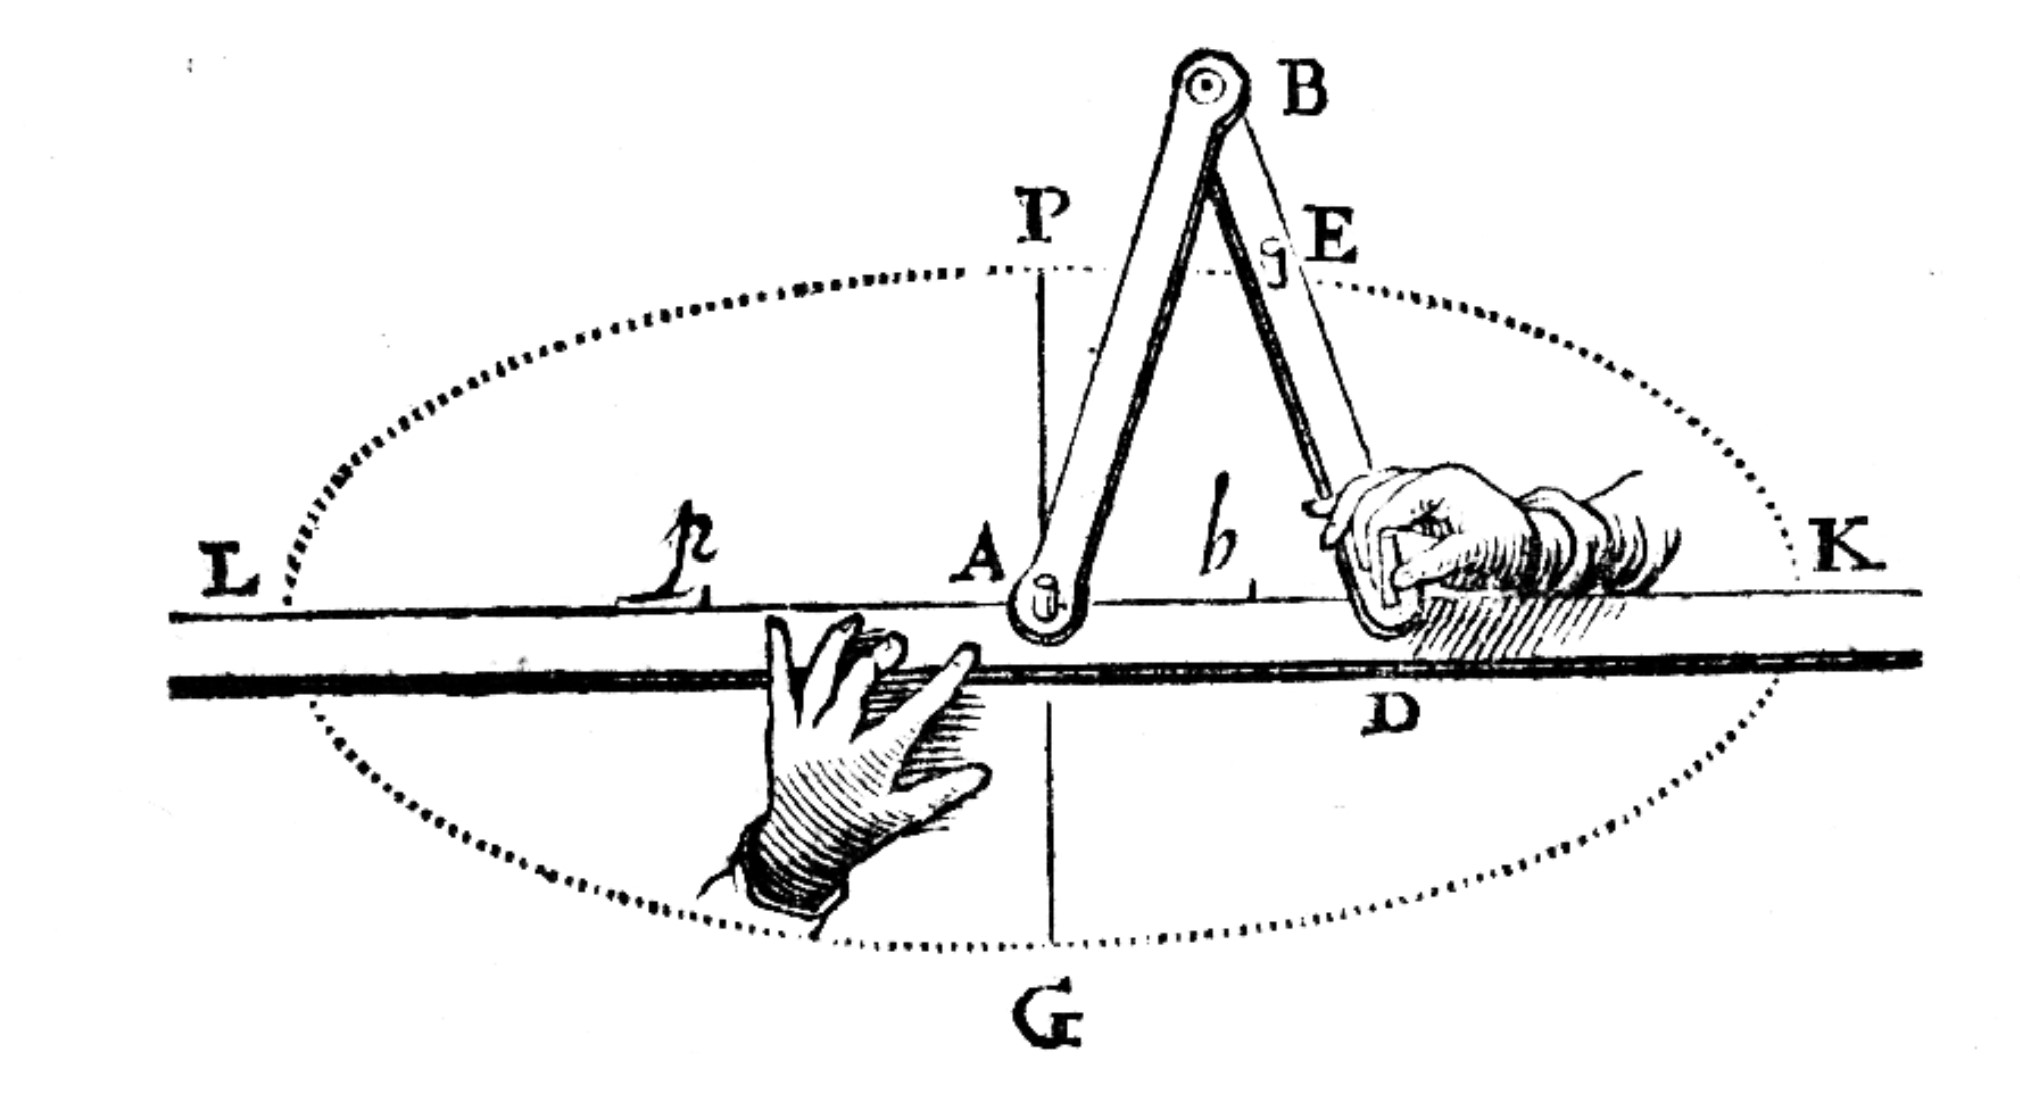
\includegraphics[width=.48\textwidth,keepaspectratio=true]{vanschooten1.jpg}
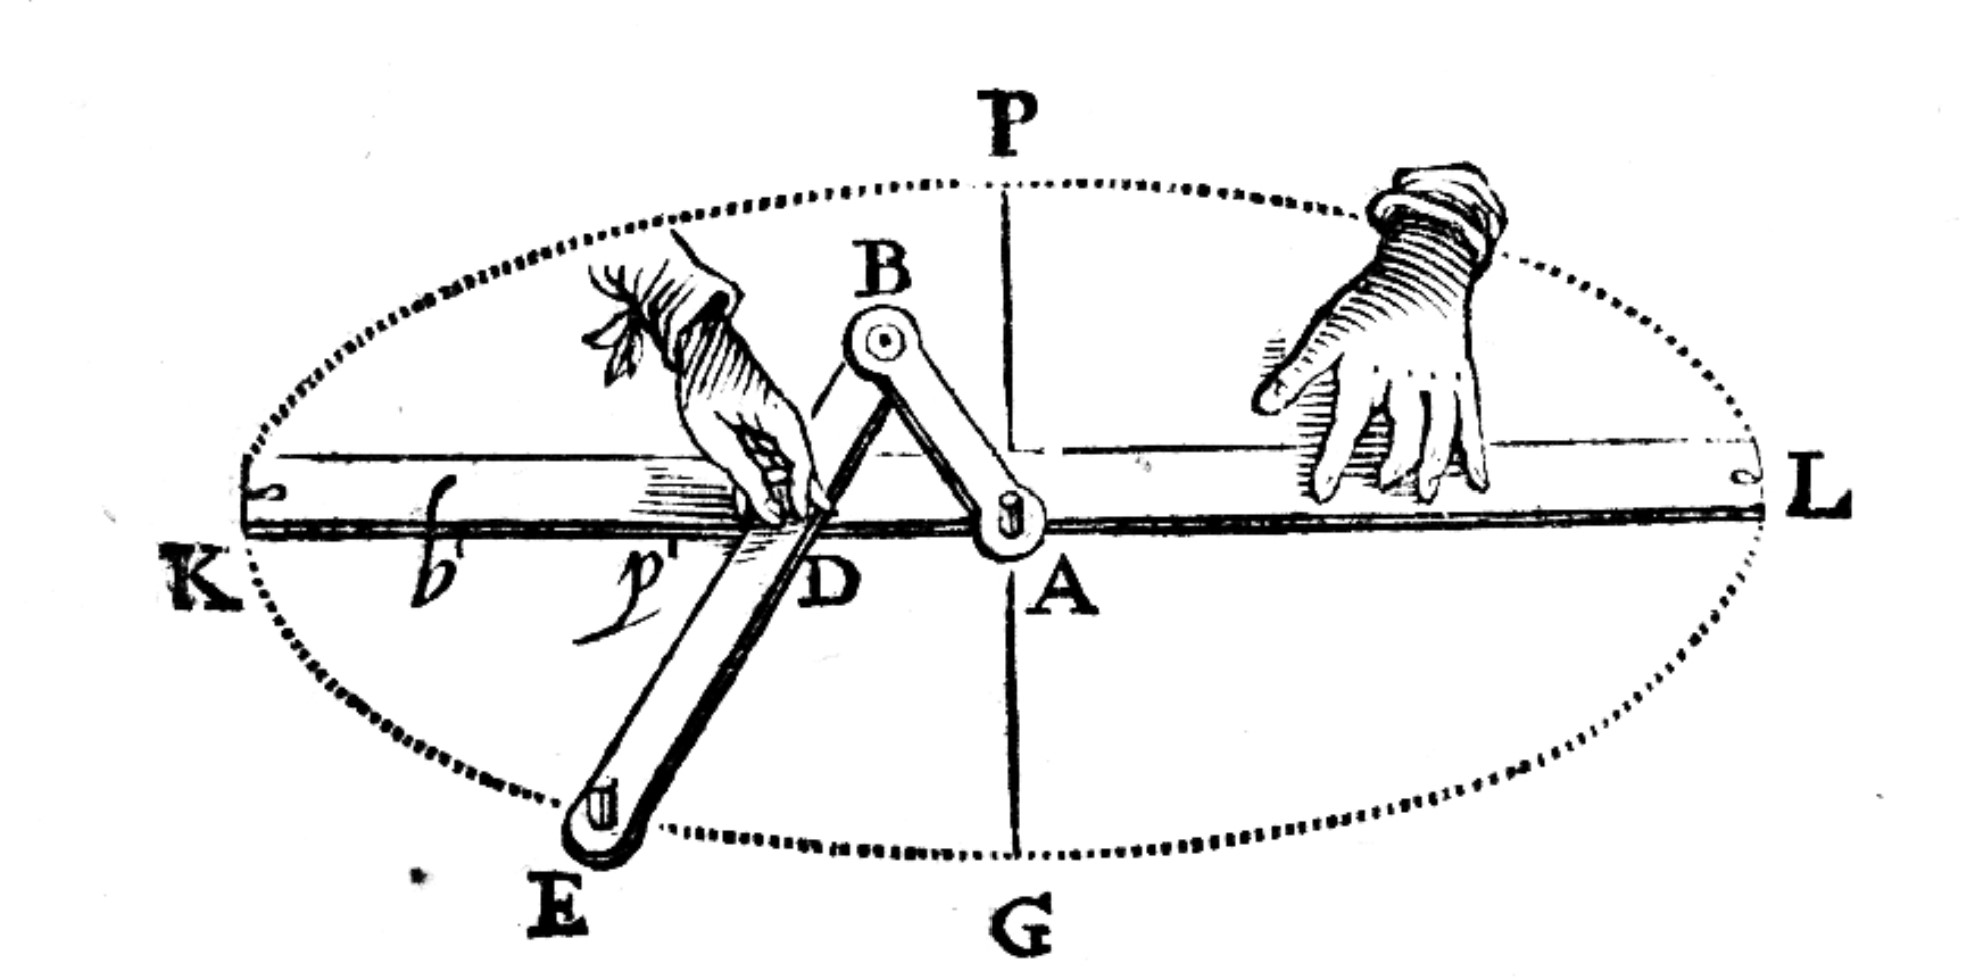
\includegraphics[width=.48\textwidth,keepaspectratio=true]{vanschooten2.jpg}
%\caption{Van Schooten's glissettes}\label{f.van-schooten}
\end{center}
%\end{figure}

\subsection*{First glissette}

Given $a,b$ let $ABD$ be an articulated arm of length $a+b$ with a rotating joint at its midpoint $B$. $D$ can slide on the $x$-axis $AK$ while $A$ can rotate at the origin (Figure~\ref{f.articulated1}). Let $E$ be at a fixed distance $b$ from $D$. Using parametric equations, we have that the locus of $E$ is an ellipse.
\begin{eqn}
PE&=&\left[ \frac{a+b}{2}+\left(\frac{a+b}{2}-b\right)\right]\cdot \cos \alpha=a\cos \alpha\\
RE&=&b\sin\alpha\,.
\end{eqn}

%%%%%%%%%%%%%%%%%%%%%%%%%%%%%%%%%%%%%%%%%%%%%%%%%%%%%%%%%%%%%%%%%%%%%%%%

\begin{figure}
\begin{center}
\begin{tikzpicture}[scale=.6]
\clip (-5.5,-1.1) rectangle +(15,8.5);

\def\a{8}
\def\b{2}
\def\ab2{5}
\def\angle{40}

\coordinate (O) at (0,0);
\coordinate (AP) at ({-\ab2},0);
\coordinate (A) at ({\ab2},0);
\coordinate (B) at (0,{\ab2});
%\node[below] at (AP) {$AP$};
\draw[name path=major] (AP) -- (A);
\path (O) -- node[below]  {$\frac{a+b}{2}$} (A);
\draw[name path=minor,thick,dashed] (O) -- ($(O)!1.4!(B)$);
\draw (AP) arc[start angle=180,end angle=0,radius={\ab2}];

\draw[blue,thick] (O) -- 
  node[above,black,yshift=2pt] {$\frac{a+b}{2}$} ({\angle}:{\ab2}) coordinate (M);

\path[name path=circle] (M) circle[radius={\ab2}];
\draw[name path=xaxis] (O) -- ($(O)!2!(A)$);
\path [name intersections = {of = xaxis and circle, by = {dummy,N} }];
\draw[red,thick] (N) -- node[above,black,yshift=2pt] {$\frac{a+b}{2}$} (M);
\draw (M) -- node[above,yshift=2pt] {$\frac{a+b}{2}$} ($(N)!2!(M)$) coordinate (L);

\draw (O) rectangle +(8pt,8pt);
\draw[very thick,red] (N) --
  node[above,black,xshift=2pt] {$b$} ($(N)!{2/5}!(M)$) coordinate (P);
\fill ($(N)+(-4pt,-2pt)$) rectangle +(8pt,4pt);

\draw[thick,dashed] (P) -- ($(L)!(P)!(O)$) node[black,left] {$Q$};
\draw[thick,dashed] (P) -- ($(A)!(P)!(O)$) node[black,below] {$R$};
\node[left,xshift=-10pt,yshift=6pt] at (N) {$\alpha$};
\node[left,xshift=-10pt,yshift=6pt] at (P) {$\alpha$};

\node[below] at (O) {$A$};
\node[above right] at (P) {$E$};
%\node[below] at (A) {$A$};
\node[above right] at (M) {$B$};
\node[below] at (N) {$D$};
%\node[left] at (L) {$L$};
\vertexsmcolor{P}{red};
\draw[very thick] (M) circle[radius=3pt];
\draw[very thick] (O) circle[radius=3pt];

\end{tikzpicture}
\caption{Constructing an ellipse with an articulated glissette (1)}\label{f.articulated1}
\end{center}
\end{figure}

%%%%%%%%%%%%%%%%%%%%%%%%%%%%%%%%%%%%%%%%%%%%%%%%%%%%%%%%%%%%%%%%%%%%%%%%

\begin{figure}[b]
\begin{center}
\begin{tikzpicture}[scale=.8]
\clip (-9,-2.7) rectangle +(18,5.4);

\def\a{5}
\def\b{3}
\def\angle{130}

\coordinate (O) at (0,0);
\node[below right] at (O) {$A$};
\coordinate (APX) at ({-\a-\b},0);
\coordinate (AX) at ({\a+\b},0);
\coordinate (BX) at (0,{\b-\a});
\coordinate (BPX) at (0,{\a-\b});
\node[left] at (APX) {$K$};
\node[right] at (AX) {$L$};
\draw[name path=major] (APX) -- (AX);
\draw[name path=minor] (BPX) -- (BX);

\draw[very thick,dotted,name path=ellipse] (O)
  ellipse[x radius={\a+\b},y radius= {\b-\a}];

\coordinate (D) at ({-0.6*\a},0);

\path[name path=arm1] (O) -- +({\angle}:3);
\path[name path=arm2] (D) -- +({180-\angle}:3);
\path [name intersections = {of = arm1 and arm2, by = {B} }];
\draw [thick,blue] (O) -- node[right,black,xshift=2pt] {$a$} (B);
\draw[thick,red] (B) -- node[left,black,xshift=-2pt] {$a$} (D);
\path [name path=arm3] (B) -- ($(B)!2.5!(D)$);
\path [name intersections = {of = arm3 and ellipse, by = {E} }];
\draw [thick,red] (D) -- node[right,black,xshift=4pt] {$b-a$} (E);

\fill ($(D)+(-4pt,-2pt)$) rectangle +(8pt,4pt);
\draw[thick,dashed] (B) -- ($(O)!(B)!(D)$) coordinate (H);
\draw[thick,dashed] (E) -- ($(O)!(E)!(D)$) coordinate (N);

\node[above] at (N) {$N$};
\node[below] at (H) {$H$};
\node[below right] at (O) {$A$};
\node[above,yshift=4pt] at (B) {$B$};
\node[below right] at (D) {$D$};
\node[below left] at (E) {$E$};

\draw (H) rectangle +(6pt,6pt);
\draw[rotate=-90] (N) rectangle +(6pt,6pt);

\node[above left,xshift=-6pt] at (O) {$\alpha$};
\node[above right,xshift=6pt] at (D) {$\alpha$};
\node[below left,xshift=-6pt] at (D) {$\alpha$};
\vertexsmcolor{E}{red};
\draw[very thick] (O) circle[radius=3pt];
\draw[very thick] (B) circle[radius=3pt];

\end{tikzpicture}
\caption{Constructing an ellipse with an articulated glissette (2)}\label{f.articulated2}
\end{center}
\end{figure}

%%%%%%%%%%%%%%%%%%%%%%%%%%%%%%%%%%%%%%%%%%%%%%%%%%%%%%%%%%%%%%%%%%%%%%%%

\subsection*{Second glissette}

Given $a,b$ let $ABE$ be an articulated arm of length $a+b$ with a rotating joint at $B$, where $AB=a, BE=b$. $D$, the intersection of $BE$ with the $x$-axis, can slide on the $x$-axis while $A$ can rotate at the origin (Figure~\ref{f.articulated2}). The locus of $E$ is an ellipse. Since $AB=AD=a$, $\angle BAD=\angle BDA=\alpha$ and $\angle NDE=\alpha$ by vertical angles. Therefore, the coordinates of $E=(x,y)$ are
\begin{eqn}
E &=& (-2a\cos \alpha - (b-a) \cos \alpha, (b-a)\sin \alpha)\\
&=& (-(a+b)\cos \alpha, b\sin\alpha)\,,
\end{eqn}
and a simple computation shows that 
\[
\frac{x^2}{(a+b)^2} + \frac{y^2}{(b-a)^2}=1\,,
\]
so $E$ is a point on an ellipse with semi-major axis $a+b$ and semi-minor axis $b-a$.

\newpage

\section{A triangle glissette}\label{s.triangle-glissette}

An ellipse can be drawing by sliding a given triangle $\triangle AQB$ along perpendicular lines $OA,OB$ (Figure~\ref{f.triangle1}). Let $OC$ be the midpoint of $AB$ and extend $OC$ so that $CP=CQ=b$. Since $\triangle AOB$ is a right triangle, $OC=AC=BC=a$. The locus of $P$ is a circle with radius $OC+CP=OC+CQ=a+b$.

%%%%%%%%%%%%%%%%%%%%%%%%%%%%%%%%%%%%%%%%%%%%%%%%%%%%%%%%%%%%%%%%%%%%%%%%

\begin{figure}[t]
\begin{center}
\begin{tikzpicture}[scale=.7]
\clip (-1,-.8) rectangle +(8,9.2);

\def\b{8}
\def\a{sqrt(100-\b*\b)}
\def\anglea{30}
\def\angleb{15}

\coordinate (O) at (0,0);
\coordinate (A) at ({\a},0);
\coordinate (B) at ({0,\b});

\path[name path=a,blue] (A) -- +({180-atan2(\b,\a)-\anglea}:8);
\path[name path=b,red] (B) -- +({-90+atan2(\a,\b)+\angleb}:10);
\path [name intersections = {of = a and b, by = {Q} }];

\coordinate (C) at ($(A)!.5!(B)$);

\draw (B) -- node[below,xshift=-2pt,yshift=-2pt] {$a$} (C) -- 
             node[below,xshift=-2pt,yshift=-2pt] {$a$} (A) --
            (O) -- (B) -- (Q) -- (A);

\path
  let
    \p1 = ($(Q) - (C)$),
    \n1 = {veclen(\x1, \y1)},
    \p2 = ($(O) - (C)$),
    \n2 = {veclen(\x2, \y2)}
  in 
    (O) -- ($(O) ! \n1+\n2 ! (C)$) coordinate (P);

\draw (O) -- node[above,yshift=2pt] {$a$} (C);
\draw (P) -- node[above,xshift=0pt,yshift=2pt] {$b$} (C) -- 
             node[below,xshift=0pt,yshift=0pt] {$b$} (Q);

\node[below] at (A) {$A$};
\node[left] at (B) {$B$};
\node[below] at (O) {$O$};
\node[right] at (P) {$P$};
\node[right] at (Q) {$Q$};
\node[left] at (C) {$C$};

\draw[red,thick] (B) -- (A) -- (Q) -- cycle;

\vertexsm{P};
\vertexsmcolor{Q}{red};
\fill ($(B)+(-1.5pt,-3pt)$) rectangle +(3pt,6pt);
\fill ($(A)+(-3pt,-1.5pt)$) rectangle +(6pt,3pt);

\end{tikzpicture}
\caption{Constructing an ellipse from the glissette triangle (red)}\label{f.triangle1}
\end{center}
\end{figure}

%%%%%%%%%%%%%%%%%%%%%%%%%%%%%%%%%%%%%%%%%%%%%%%%%%%%%%%%%%%%%%%%%%%%%%%%

Figure~\ref{f.triangle2} shows that as $B$ slides down and $A$ slides right, $CQ$ rotates upwards while $OC$ rotates downwards. By considering the extremes ($A$ near $O$ and $B$ near $O$), it is clear that $OCQ$ will be ``concave'' up at one extreme and ``concave'' down at the other. Therefore, there must be a position of $AB$ which $OCQ$ is a line segment (green).

%%%%%%%%%%%%%%%%%%%%%%%%%%%%%%%%%%%%%%%%%%%%%%%%%%%%%%%%%%%%%%%%%%%%%%%%

\begin{figure}[b]
\begin{center}
\begin{tikzpicture}[scale=.8]
\clip (-.5,-.6) rectangle +(10.2,8.8);

\def\b{8}
\def\a{sqrt(100-\b*\b)}
\def\anglea{30}
\def\angleb{20}
\coordinate (O) at (0,0);
\coordinate (A) at ({\a},0);
\coordinate (B) at ({0,\b});
\path[name path=a,blue] (A) -- +({180-atan2(\b,\a)-\anglea}:8);
\path[name path=b,red] (B) -- +({-90+atan2(\a,\b)+\angleb}:10);
\path [name intersections = {of = a and b, by = {Q} }];
\draw[thick,dotted] (A) -- (B) -- (Q) -- cycle;
\draw (A) -- (O) -- (B);
\fill ($(B)+(-1.5pt,-3pt)$) rectangle +(3pt,6pt);
\fill ($(A)+(-3pt,-1.5pt)$) rectangle +(6pt,3pt);
\coordinate (C) at ($(A)!.5!(B)$);
\draw
  let
    \p1 = ($(Q) - (C)$),
    \n1 = {veclen(\x1, \y1)},
    \p2 = ($(O) - (C)$),
    \n2 = {veclen(\x2, \y2)}
  in 
    (O) -- ($(O) ! \n1+\n2 ! (C)$) coordinate (P);
\node[right] at (P) {$P$};
\draw[thick,red] (O) node[below,black] {$O$} -- 
  (C) node[left,black] {$C$} -- (Q) node[right,black] {$Q$};
\fill[shift only,red] (P) circle (2pt);

\def\b{3}
\def\a{sqrt(100-\b*\b)}
\def\anglea{30}
\def\angleb{20}
\coordinate (O) at (0,0);
\coordinate (A) at ({\a},0);
\coordinate (B) at ({0,\b});
\path[name path=a,blue] (A) -- +({180-atan2(\b,\a)-\anglea}:8);
\path[name path=b,red] (B) -- +({-90+atan2(\a,\b)+\angleb}:10);
\path [name intersections = {of = a and b, by = {Q} }];
\draw[thick,dotted] (A) -- (B) -- (Q) -- cycle;
\draw (A) -- (O) -- (B);
\fill ($(B)+(-1.5pt,-3pt)$) rectangle +(3pt,6pt);
\fill ($(A)+(-3pt,-1.5pt)$) rectangle +(6pt,3pt);
\coordinate (C) at ($(A)!.5!(B)$);
\draw
  let
    \p1 = ($(Q) - (C)$),
    \n1 = {veclen(\x1, \y1)},
    \p2 = ($(O) - (C)$),
    \n2 = {veclen(\x2, \y2)}
  in 
    (O) -- ($(O) ! \n1+\n2 ! (C)$) coordinate (P);
\node[right,xshift=8pt,yshift=2pt] at (P) {$P$};
\draw[thick,blue] (O) -- (C) node[below,black] {$C$} --  
  (Q) node[right,black,xshift=5pt] {$Q$};
\fill[shift only,blue] (P) circle (2pt);

\def\b{5}
\def\a{sqrt(100-\b*\b)}
\def\anglea{30}
\def\angleb{20}
\coordinate (O) at (0,0);
\coordinate (A) at ({\a},0);
\coordinate (B) at ({0,\b});
\path[name path=a,blue] (A) -- +({180-atan2(\b,\a)-\anglea}:8);
\path[name path=b,red] (B) -- +({-90+atan2(\a,\b)+\angleb}:10);
\path [name intersections = {of = a and b, by = {Q} }];
\draw[thick,dotted] (A) -- (B) -- (Q) -- cycle;
\draw (A) -- (O) -- (B);
\fill ($(B)+(-1.5pt,-3pt)$) rectangle +(3pt,6pt);
\fill ($(A)+(-3pt,-1.5pt)$) rectangle +(6pt,3pt);
\coordinate (C) at ($(A)!.5!(B)$);
%\node[right,xshift=10pt,yshift=1pt] at (Q) {$P$};
\draw[thick,green!80!black] (O) -- 
  (C) node[above,black] {$C$} --
  (Q) node[right,black] {$Q,P$};
\fill[shift only,green!80!black] (Q) circle (2pt);

\end{tikzpicture}
\caption{There are $A,B$ such that $OCQ$ is a line segment (green)}\label{f.triangle2}
\end{center}
\end{figure}

%%%%%%%%%%%%%%%%%%%%%%%%%%%%%%%%%%%%%%%%%%%%%%%%%%%%%%%%%%%%%%%%%%%%%%%%

Referring now to Figure~\ref{f.triangle3}, let $OQ'$ is the straight line segment and let $C,Q,P$ are points generated by another arbitrary position of $AB$. Construct $CE\parallel OQ'$ which bisects $\angle PCQ$ since $CP=CQ$, and construct $PN\perp OQ'$ and $CL\perp OQ'$.

From $\triangle OCL\sim \triangle CPE$ we have
\begin{eqnarray*}
\frac{CL}{PE}&=&\frac{OC}{CP}\\[4pt]
\frac{CL}{PE}-\frac{PE}{PE}&=&\frac{OC}{CP}-\frac{CP}{CP}\\[4pt]
\frac{CL-PE}{PE}&=&\frac{OC-CP}{CP}\,,
\end{eqnarray*}
and similarly,
\[
\frac{CL+PE}{PE}=\frac{OC+CP}{CP}\,.
\]
Now,
\begin{eqnarray*}
QN &=& EN - EQ = CL - PE\\
PN &=& EN + PE = CL + PE\\[4pt]
\frac{QN}{PN}&=& \frac{CL-PE}{CL+PE}=\frac{OC-CP}{OC+CP}\,.
\end{eqnarray*}
By Theorem~\ref{thm.ellipse-b-over-a-besant}, the locus of $Q$ is an ellipse with $OC+CQ=a+b$ the semi-major axis and $OC-CQ=a-b$ the semi-minor axis.

%%%%%%%%%%%%%%%%%%%%%%%%%%%%%%%%%%%%%%%%%%%%%%%%%%%%%%%%%%%%%%%%%%%%%%%%

\begin{figure}[t]
\begin{center}
\begin{tikzpicture}[scale=.85]
\clip (-.5,-.6) rectangle +(8,7);

\def\b{8}
\def\a{sqrt(100-\b*\b)}
\def\anglea{30}
\def\angleb{20}
\coordinate (O) at (0,0);
\coordinate (A) at ({\a},0);
\coordinate (B) at ({0,\b});
\path[name path=a,blue] (A) -- +({180-atan2(\b,\a)-\anglea}:8);
\path[name path=b,red] (B) -- +({-90+atan2(\a,\b)+\angleb}:10);
\path [name intersections = {of = a and b, by = {Q} }];
\coordinate (C) at ($(A)!.5!(B)$);
\draw
  let
    \p1 = ($(Q) - (C)$),
    \n1 = {veclen(\x1, \y1)},
    \p2 = ($(O) - (C)$),
    \n2 = {veclen(\x2, \y2)}
  in 
    (O) -- ($(O) ! \n1+\n2 ! (C)$) coordinate (P);
\node[right] at (P) {$P$};
\draw[thick,red] (O) node[below,black] {$O$} -- 
  (C) node[left,black] {$C$} -- (Q) node[right,black] {$Q$};

\def\b{5}
\def\a{sqrt(100-\b*\b)}
\def\anglea{30}
\def\angleb{20}
\coordinate (O) at (0,0);
\coordinate (A) at ({\a},0);
\coordinate (B) at ({0,\b});
\path[name path=a,blue] (A) -- +({180-atan2(\b,\a)-\anglea}:8);
\path[name path=b,red] (B) -- +({-90+atan2(\a,\b)+\angleb}:10);
\path [name intersections = {of = a and b, by = {QX} }];
\coordinate (CX) at ($(A)!.5!(B)$);
\draw[thick,green!80!black] (O) -- 
  (CX) --% node[below,black] {$[C]$} --
  (QX) node[right,black] {$Q'$};

\draw (C) -- ($(O)!(C)!(CX)$) coordinate (L);
\node[below,xshift=2pt,yshift=-2pt] at (L) {$L$};
\draw (P) -- ($(O)!(P)!(QX)$) coordinate (N);
\node[below,xshift=2pt,yshift=-2pt] at (N) {$N$};
\draw (C) -- ($(P)!(C)!(N)$) coordinate (E);
\node[right,xshift=0pt,yshift=0pt] at (E) {$E$};

\node[above right,xshift=10pt,yshift=9pt] at (C) {$\alpha$};
\node[above right,xshift=14pt,yshift=2pt] at (C) {$\alpha$};

\draw[rotate=120] (L) rectangle +(6pt,6pt);
\draw[rotate=124] (N) rectangle +(6pt,6pt);
\draw[rotate=120] (E) rectangle +(6pt,6pt);
\end{tikzpicture}
\caption{$OQ'$ is the line segment and $C,Q$ are for another arbitrary position of $AB$}\label{f.triangle3}
\end{center}
\end{figure}

%%%%%%%%%%%%%%%%%%%%%%%%%%%%%%%%%%%%%%%%%%%%%%%%%%%%%%%%%%%%%%%%%%%%%%%%

\section{Confocal ellipses}\label{s.confocal}

\emph{Confocal ellipses} are ellipses with the same foci. Given an ellipse $E$, a confocal ellipse can be drawn using a modification of the gardener method. If the length of the major axis of $E$ is $2a$, take a rope of length greater than $2a$, wrap it around $E$ and pull taut with a pencil. As you move around $E$, the pencil will trace a confocal ellipse (Figure~\ref{f.confocal1}).

\begin{figure}[t]
\begin{center}
\begin{tikzpicture}[scale=.75]

\clip (-4.2,-2.2) rectangle +(8.5,6.5);

% Size and center of the ellipse
\def\a{4}
\def\b{2}
\def\angle{30}

\pic{ellipse={3*\a/4}/{3*\b/4}};  % Scale
\coordinate (P) at ({\angle}:{\a} and {\b});
\draw[white] (Top) -- (Bot);
\draw[white] (Left) -- (Right);
\path[name path global=t1] 
  (P) -- ++ ({-2*\a*sin(\angle)},{2*\b*cos(\angle)});

\coordinate (D) at ({\angle+120}:{\a} and {\b});
\path[name path global=t2] 
  (D) -- ++ ({2*\a*sin(\angle+120)},{-2*\b*cos(\angle+120)});

\path [name intersections = {of = t1 and t2, by = {Q}}];
\draw [thick,red] (D) -- (Q) -- (P);
\draw[thick] (Q) circle[radius=3pt];

\draw[thick,red] (P) 
        arc[start angle=30,end angle=-210, x radius=\a,y radius=\b];

\end{tikzpicture}
\caption{Gardner's method for constructing a confocal ellipse}\label{f.confocal1}
\end{center}
\end{figure}

To prove that the locus is an ellipse, let the tip of the pencil be at $T$ and very soon after let it be at $t$.\footnote{The proof is from the solution for problem 46 in the 1890 edition of Besant \url{https://archive.org/details/solutionsexampl00besagoog}, with details supplied by ``Intelligenti pauca'' at \url{https://math.stackexchange.com/questions/4908340/besants-proof-of-graves-theorem}.}
The string forms two pairs of tangents $PT,TQ$ and $pt,tq$. Now $PT\approx pt$ so
\begin{eqn}
PT&\approx&\widehat{Pp} +PV \approx \widehat{Pp} + pt-tV\\
tV&\approx& \widehat{Pp} + pt - PT\,.
\end{eqn}

%%%%%%%%%%%%%%%%%%%%%%%%%%%%%%%%%%%%%%%%%%%%%%%%%%%%%%%%%%%%%%%%%%%%%%%%

\begin{figure}[b]
\begin{center}
\begin{tikzpicture}[scale=1]

\clip (-6.5,2) rectangle +(13,4.5);

% Size and center of the ellipse
\def\a{7}
\def\b{4}

\coordinate (O) at (0,0);
\draw[name path global=ellipse] (0,0) ellipse [x radius=\a,y radius=\b];

\def\anglep{140}
\def\angleq{50}
\def\anglepp{130}
\def\angleqp{40}

\coordinate (P) at ({\anglep}:{\a} and {\b});
\path[name path global=tp] 
  (P) -- ++ ({1.8*\a*sin(\anglep)},{-1.8*\b*cos(\anglep)});
\coordinate (Q) at ({\angleq}:{\a} and {\b});
\path[name path global=tq] 
  (Q) -- ++ ({-1.8*\a*sin(\angleq)},{1.8*\b*cos(\angleq)});
\path [name intersections = {of = tp and tq, by = {T}}];
\draw (P) -- (T) -- (Q);

\coordinate (PP) at ({\anglepp}:{\a} and {\b});
\path[name path global=tpp] 
  (PP) -- ++ ({1.5*\a*sin(\anglepp)},{-1.5*\b*cos(\anglepp)});
\coordinate (QP) at ({\angleqp}:{\a} and {\b});
\path[name path global=tqp] 
  (QP) -- ++ ({-1.5*\a*sin(\angleqp)},{1.5*\b*cos(\angleqp)});
\path [name intersections = {of = tpp and tqp, by = {TP}}];
\draw (PP) -- (TP) -- (QP);

\draw (T) -- ($(PP)!(T)!(TP)$) coordinate (V);
\draw (TP) -- ($(T)!(TP)!(Q)$) coordinate (VP);

\draw[rotate=29] (V) rectangle +(5pt,5pt);
\draw[rotate=-30] (VP) rectangle +(5pt,5pt);

\node[above] at (T) {$T$};
\node[above] at (P) {$P$};
\node[above] at (TP) {$t$};
\node[below] at (PP) {$p$};
\node[below] at (V) {$V$};
\node[below] at (VP) {$y$};
\node[above] at (Q) {$Q$};
\node[right] at (QP) {$q$};

\vertexsm{P};
\vertexsm{PP};
\vertexsm{Q};
\vertexsm{QP};

\end{tikzpicture}
\caption{Constructing a confocal ellipse}\label{f.confocal}
\end{center}
\end{figure}

%%%%%%%%%%%%%%%%%%%%%%%%%%%%%%%%%%%%%%%%%%%%%%%%%%%%%%%%%%%%%%%%%%%%%%%%

Similarly,
\begin{eqn}
tq&\approx& \widehat{Qq} + QT - Ty\\
Ty&\approx& \widehat{Qq} + QT - tq\,.
\end{eqn}
Since the length of the string is fixed, $PT+TQ = pt+tq$ and $\widehat{Pp}\approx\widehat{Qq}$. Substituting into the above equations gives
\[
tV= \widehat{Pp} + pt - PT \approx \widehat{Pp} + TQ -tq\approx
\widehat{Qq} + QT - tq\approx Ty\,.
\]

Consider now Figure~\ref{f.confocal-details} which is a detail from Firgure~\ref{f.confocal}. The angles $\alpha$ are vertical angles and we showed that $TV\approx ty$ so $\triangle TVW\cong \triangle tyW$. Therefore, $\triangle TVt\cong tyT$ and $\angle TtW=\angle tTW=\beta$.  What happens as $t$ approaches $T$ each other? $tT$ becomes the ``left'' part of the tangent at $T$ and $Tt$ becomes the ``right'' part of the tangent. It follows by Theorem~\ref{thm.tangent-angles} that there is a tangent of an ellipse at $T$.

%%%%%%%%%%%%%%%%%%%%%%%%%%%%%%%%%%%%%%%%%%%%%%%%%%%%%%%%%%%%%%%%%%%%%%%%

\begin{figure}
\begin{center}
\begin{tikzpicture}[scale=3]

\clip (-1.5,4.5) rectangle +(3,1.3);

% Size and center of the ellipse
\def\a{7}
\def\b{4}

\coordinate (O) at (0,0);
\draw[name path global=ellipse] (0,0) ellipse [x radius=\a,y radius=\b];

\def\anglep{140}
\def\angleq{50}
\def\anglepp{130}
\def\angleqp{40}

\coordinate (P) at ({\anglep}:{\a} and {\b});
\path[name path global=tp] 
  (P) -- ++ ({1.8*\a*sin(\anglep)},{-1.8*\b*cos(\anglep)});
\coordinate (Q) at ({\angleq}:{\a} and {\b});
\path[name path global=tq] 
  (Q) -- ++ ({-1.8*\a*sin(\angleq)},{1.8*\b*cos(\angleq)});
\path [name intersections = {of = tp and tq, by = {T}}];
\draw (P) -- (T) -- (Q);

\coordinate (PP) at ({\anglepp}:{\a} and {\b});
\path[name path global=tpp] 
  (PP) -- ++ ({1.5*\a*sin(\anglepp)},{-1.5*\b*cos(\anglepp)});
\coordinate (QP) at ({\angleqp}:{\a} and {\b});
\path[name path global=tqp] 
  (QP) -- ++ ({-1.5*\a*sin(\angleqp)},{1.5*\b*cos(\angleqp)});
\path [name intersections = {of = tpp and tqp, by = {TP}}];
\draw (PP) -- (TP) -- (QP);

\draw (T) -- ($(PP)!(T)!(TP)$) coordinate (V);
\draw (TP) -- ($(T)!(TP)!(Q)$) coordinate (VP);

\draw[rotate=26] (V) rectangle +(2pt,2pt);
\draw[rotate=63] (VP) rectangle +(2pt,2pt);

\node[above] at (T) {$T$};
\node[above] at (P) {$P$};
\node[above] at (TP) {$t$};
\node[below] at (PP) {$p$};
\node[below] at (V) {$V$};
\node[below] at (VP) {$y$};
\node[above] at (Q) {$Q$};
\node[right] at (QP) {$q$};

\vertexsm{P};
\vertexsm{PP};
\vertexsm{Q};
\vertexsm{QP};

\draw (T) -- (TP);
\path [name intersections = {of = tpp and tq, by = {W}}];
\node[below,yshift=-2pt] at (W) {$W$};
\node[left,xshift=-6pt] at (W) {$\alpha$};
\node[right,xshift=6pt] at (W) {$\alpha$};
\node[below right,xshift=10pt,yshift=-10pt] at (T) {$\alpha'$};
\node[below left,xshift=-10pt,yshift=-10pt] at (TP) {$\alpha'$};
\node[right,xshift=24pt,yshift=-7pt] at (T) {$\beta$};
\node[left,xshift=-24pt,yshift=-7pt] at (TP) {$\beta$};

\end{tikzpicture}
\caption{Detail of the proof for a confocal ellipse}\label{f.confocal-details}
\end{center}
\end{figure}

%%%%%%%%%%%%%%%%%%%%%%%%%%%%%%%%%%%%%%%%%%%%%%%%%%%%%%%%%%%%%

\section{The perfect compass}\label{s.perfect}

The \emph{perfect compass} is an instrument that is capable of constructing any conic section. It consists of an \emph{axis} attached to a point $A$ in the plane at an angle $\alpha$ to the plane. An \emph{arm} is attached at $B$ to the axis at an angle $\beta$ to the axis. The arm contains a pencil that can slide within the arm so that it is always in contact with the base. As the arm rotates around the axis it draws a conic section (Figures~\ref{f.perfect-image1}, ~\ref{f.perfect-image2}).\footnote{The images in the Figures are courtesy of the Associazione Macchine Matematiche. \\\hspace*{1.5em} \url{https://www.macchinematematiche.org/en/conics/compasso-perfetto.html}.\\\hspace*{1.5em} Animations of the perfect compass can be found at \url{https://www.geogebra.org/m/tMxr4Mah} and\\\hspace*{1.5em} \url{https://www.geogebra.org/m/uj2xauej}.}

The notation in the figures in the sequel conforms to the notation in \cite{henk}. $B$ denotes the point of attachment of the arm to the axis while $O$ is reserved for the center of the conic section. The axis is drawn in red and the arm in blue.

The parameters $\alpha, \beta, AB$ determine which conic section will be drawn. Here we limit ourselves to ellipses by specifying that $0< \beta <\alpha< 90$. 
\begin{figure}[h]
\begin{minipage}{.45\textwidth}
\begin{center}
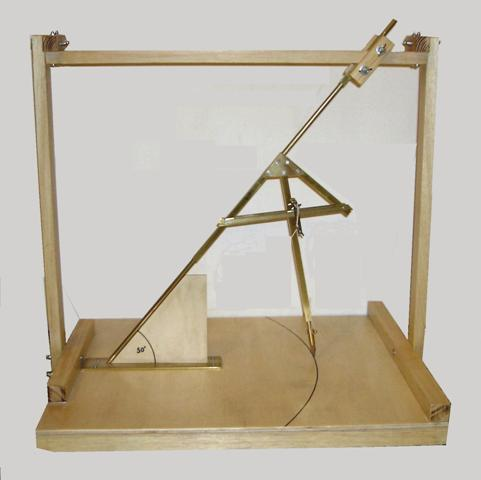
\includegraphics[width=.9\textwidth,keepaspectratio=true]{perfect1.jpg}
\medskip
\caption{A perfect compass}\label{f.perfect-image1}
\end{center}
\end{minipage}
\hfill
\begin{minipage}{.55\textwidth}
\begin{center}
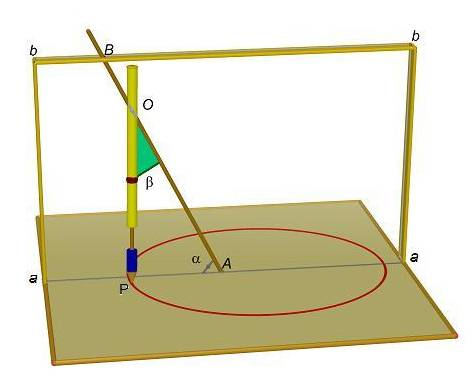
\includegraphics[width=\textwidth,keepaspectratio=true]{perfect2.jpg}
\caption{The configuration of a perfect compass}\label{f.perfect-image2}
\end{center}
\end{minipage}
\end{figure}

%\begin{figure}[h]
%\begin{center}
%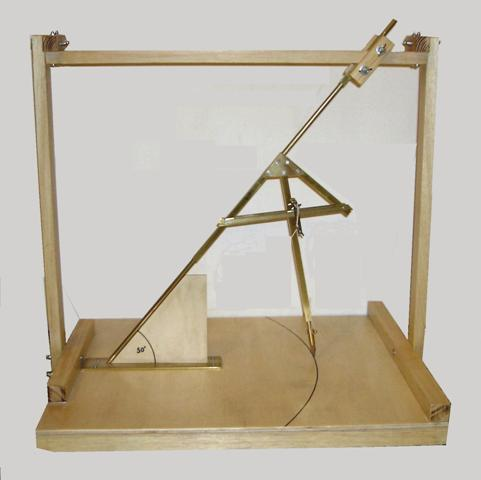
\includegraphics[width=.5\textwidth,keepaspectratio=true]{perfect1.jpg}
%\caption{A perfect compass}\label{f.perfect-image1}
%\end{center}
%\end{figure}
%\begin{figure}[h]
%\begin{center}
%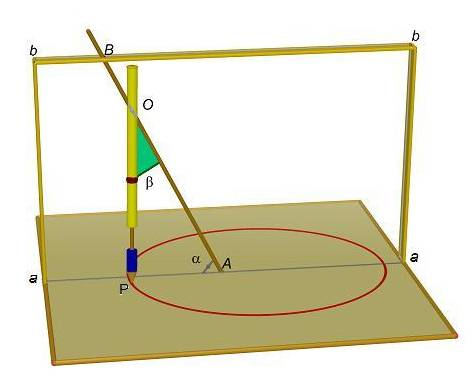
\includegraphics[width=.6\textwidth,keepaspectratio=true]{perfect2.jpg}
%\caption{The configuration of a perfect compass}\label{f.perfect-image2}
%\end{center}
%\end{figure}


%%%%%%%%%%%%%%%%%%%%%%%%%%%%%%%%%%%%%%%%%%%%%%%%%%%%%%%%%%%%%

\subsubsection*{Constructing the major axis of an ellipse}

Consider an arbitrary point $A$ on an arbitrary line $l$ that (Figure~\ref{f.perfect-major}). Place the base of the axis at $A$ and rotate the axis until the arm at $B$ intersects the line $l$. There are two such intersections labeled $E$ and $D$. Let the midpoint of $ED$ be $O$. Construct the (outer) circle centered at $O$ with radius $OD=OE=r_o$.

The diagrams will be drawn in two dimensions; you have to imagine that $B$ is actually above the plane and the axis $AB$ and the arms $BD, BE$ have been ``laid flat.''

%%%%%%%%%%%%%%%%%%%%%%%%%%%%%%%%%%%%%%%%%%%%%%%%%%%%%%%%%%%%%

\begin{figure}[b]
\begin{minipage}{.49\textwidth}
\begin{center}
\begin{tikzpicture}[scale=.8]
\clip  (-3.9,-3.6) rectangle +(9,7.2);

\def\alph{50}
\def\bet{30}
\def\len{3.5}

\path[name path=major] (-6,0) -- (10,0);
\coordinate (A) at (2,0);
\node[below right] at (A) {$A$};
\draw[thick,red] (A) --  +({\alph}:{\len}) coordinate (B);
\path[thick,name path=arm1] (B) -- +({180+\alph-\bet}:12);
\node[above] at (B) {$B$};

\path [name intersections = {of = arm1 and major, by = {E}}];
\node[below left] at (E) {$E$};

\draw[blue,thick] (B) -- (E);

\path[thick,name path=arm2] (B) -- +({180+\alph+\bet}:6);
\path [name intersections = {of = arm2 and major, by = {D}}];
\node[below right] at (D) {$D$};

\draw[blue,thick] (B) -- (D);

\coordinate (O) at ($(E)!.5!(D)$);
\node[below left] at (O) {$O$};
\node[draw,thick,dashed,name path=circle] at (O) 
  [circle through = (D)] {};
\draw ($(E)+(-36pt,0)$) -- ($(D)+(36pt,0)$) node[xshift=-2pt,above] {$l$};
\path (E) -- node[below] {$r_o$} (O);

\node[above right,xshift=3pt] at (A) {\sm{\alpha}};
\node[above left,xshift=5pt] at (A) {\sm{180\!-\!\alpha}};
\node[below left,xshift=-10pt,yshift=-5pt] at (B) {\sm{\beta}};
\node[below left,xshift=-1pt,yshift=-7pt] at (B) {\sm{\beta}};
\vertexsm{O};

\end{tikzpicture}
\caption{Constructing the major axis}\label{f.perfect-major}
\end{center}
\end{minipage}
%\end{figure}
\hfill
%\begin{figure}[t]
\begin{minipage}{.49\textwidth}
\begin{center}
\begin{tikzpicture}[scale=.8]
\clip  (-3.7,-3.6) rectangle +(9.4,7.2);

\def\alph{50}
\def\bet{30}
\def\len{3.5}

\path[name path=major] (-6,0) -- (10,0);
\coordinate (A) at (2,0);
\node[below right] at (A) {$A$};
%\draw[thick,red] (A) -- +({\alph}:{\len}) coordinate (B);
\path[thick,name path=arm1] (B) -- +({180+\alph-\bet}:12);
%\node[above] at (B) {$B$};

\path [name intersections = {of = arm1 and major, by = {E}}];
\node[below left] at (E) {$E$};

%\draw[blue,thick] (B) -- (E);
\draw (E) -- (A);

\path[thick,name path=arm2] (B) -- +({180+\alph+\bet}:6);
\path [name intersections = {of = arm2 and major, by = {D}}];
\node[below right] at (D) {$D$};

%\draw[blue,thick] (B) -- (D);

\coordinate (O) at ($(E)!.5!(D)$);
\node[below left] at (O) {$O$};
\node[draw,thick,dashed,name path=circle] at (O) 
  [circle through = (D)] {};

\draw[thick,red] (A) -- +({\len},0) coordinate (U);
\node[below] at (U) {$U$};

\path[name path=arm3] (U) -- +({180+\bet}:7);
\path[name path=perp] (A) -- +(-90:5);

\path [name intersections = {of = arm3 and perp, by = {G}}];
\node[below right] at (G) {$G$};
\draw[thick,blue] (U) -- (G);
\path [name intersections = {of = perp and circle, by = {K}}];
\node[below] at (K) {$K$};
\draw (A) -- (K);
\path[name path=ko] (O) -- (K);
\path[name path=gl] (G) -- +(180:4);
\path [name intersections = {of = ko and gl, by = {L}}];
\node[below,xshift=-3pt,yshift=-5pt] at (L) {$L$};
\draw (G) -- (L);

\node[draw,thick,dotted,name path=inner] at (O)   
  [circle through = (L)] {};

\path[name path=minor] ($(O)+(0,4)$) -- ($(O)+(0,-4)$);
\path [name intersections = {of = minor and inner, by = {H,T}}];
\node[above] at (H) {$H$};
\node[below] at (T) {$T$};

\draw (H) -- node[left] {$r_i$} (O) -- node[left] {$r_i$} (T);

\draw[very thick,cyan] (O) -- node[xshift=-3pt,below,black] {$r_i$} (L);
\draw[very thick,brown] ($(O)+(4pt,0pt)$) --
   node[above,black,xshift=4pt] {$r_o$} ($(K)+(4pt,0pt)$);

%\node[above,xshift=-3pt,yshift=5pt] at (K) {\sm{\beta}};
\node[below left,xshift=-12pt,yshift=1pt] at (U) {\sm{\beta}};
%\vertexsm{G};
%\draw[rotate=180] (G) rectangle +(5pt,5pt);
%\draw[rotate=180] (A) rectangle +(5pt,5pt);
%\draw[rotate=90] (O) rectangle +(5pt,5pt);
\end{tikzpicture}
\caption{Constructing the minor axis}\label{f.perfect-minor}
\end{center}
\end{minipage}
\end{figure}

%%%%%%%%%%%%%%%%%%%%%%%%%%%%%%%%%%%%%%%%%%%%%%%%%%%%%%%%%%%%%

\subsubsection*{Constructing the minor axis of an ellipse}

Consider now the situation where axis is rotated to $-90^\circ$ and denote by $G$ the intersection of the arm with the plane. If you lay the compass flat, the axis $AB$ becomes $U$ (Figure~\ref{f.perfect-minor}). Extend $AG$ until it intersects the circle at $K$ and construct $OK=r_o$ (brown). Construct the perpendicular to $AK$ at $G$ and let its intersection with $OK$ be $L$. Draw the (inner) circle centered at $O$ with radius $OL=r_i$ (cyan). Construct the perpendicular to $ED$ at $O$ and let its intersections with the inner circle be $H,T$.

\begin{theorem}[Prop. VIII]\label{thm.propviii}
$\displaystyle\frac{AG}{AK}=\frac{HO}{OD}$, where $HO=r_i$ and $OD=r_o$ are the semi-minor and semi-major axes of an ellipse.
\end{theorem}
\begin{proof}
By Theorem~\ref{thm.ratios-besant},
\[
\frac{AG^2}{DA\cdot AE} = \frac{HO^2}{OD^2}\,,
\]
and by Theorem~\ref{thm.alt-hypo}, $AK^2=DA\cdot AE$ .\hqed
\end{proof}

\subsubsection*{$G$ is a point on the ellipse}

\begin{theorem}
$G$ is a point on the ellipse with semi-major axis $r_o$ and semi-minor axis $r_i$
\end{theorem}
\begin{proof}(Proof 1)
Since $\triangle AKO \sim \triangle AGO$, by Theorem~\ref{thm.propviii},
\[
\frac{AG}{AK}=\frac{OL}{OK}=\frac{r_i}{r_o}=\frac{HO}{OD}\,,
\]
and $G$ is a point on an ellipse with semi-minor axis $r_i$ and semi-major axis $r_o$.\hqed
\end{proof}

%%%%%%%%%%%%%%%%%%%%%%%%%%%%%%%%%%%%%%%%%%%%%%%%%%%%%%%%%%%%%

\begin{proof}(Proof 2)
$G$ will be on the ellipse if its coordinates satisfy the parametric representation (Definition~\ref{def.parametric}). Let $t$ be the angle between $OD$ and $OK$. $OA=r_o\cos t$ and $AG=r_i\sin t$ (Figure~\ref{f.perfect-parametric}), so $G$ is a point on the ellipse. \hqed
\end{proof}

Figure~\ref{f.perfect-ellipse} shows the ellipse (green) and you can check that $G$ is on the ellipse. It also shows that a symmetric construction gives the point $G'$ on the ellipse. Another symmetric construction shows that there are an additional pair of points to the left of the minor-axis.  We have now located six points on an ellipse. From the following surprising theorem (proof omitted) we conclude that the perfect compass constructs an ellipse.\footnote{Approaches to proving the theorem are discussed in the Wikipedia article \emph{Five points determine a conic}.}

\begin{theorem}
Given five points, no three of which are collinear, there is a unique conic section containing the points.
\end{theorem}


%%%%%%%%%%%%%%%%%%%%%%%%%%%%%%%%%%%%%%%%%%%%%%%%%%%%%%%%%%%%%

\begin{figure}
\begin{minipage}{.49\textwidth}
\begin{center}
\begin{tikzpicture}[scale=.8]
\clip (-3.8,-3.6) rectangle +(8.4,7.2);

\def\alph{50}
\def\bet{30}
\def\len{3.5}

\path[name path=major] (-6,0) -- (10,0);
\coordinate (A) at (2,0);
\node[below right] at (A) {$A$};
%\draw[thick,red] (A) -- +({\alph}:{\len}) coordinate (B);
\path[thick,name path=arm1] (B) -- +({180+\alph-\bet}:12);
%\node[above] at (B) {$B$};

\path [name intersections = {of = arm1 and major, by = {E}}];
\node[below left] at (E) {$E$};

%\draw[blue,thick] (B) -- (E);
\draw (E) -- (D);

\path[thick,name path=arm2] (B) -- +({180+\alph+\bet}:6);
\path [name intersections = {of = arm2 and major, by = {D}}];
\node[below right] at (D) {$D$};

\coordinate (O) at ($(E)!.5!(D)$);
\node[below left] at (O) {$O$};
\node[draw,thick,dashed,name path=circle] at (O) 
  [circle through = (D)] {};

\path[name path=arm3] (U) -- +({180+\bet}:7);
\path[name path=perp] (A) -- +(-90:5);

\path [name intersections = {of = arm3 and perp, by = {G}}];
\node[below right] at (G) {$G$};
%\draw[thick,blue] (U) -- (G);
\path [name intersections = {of = perp and circle, by = {K}}];
\node[below] at (K) {$K$};
\draw (A) -- (K);
\path[name path=ko] (O) -- (K);
%\draw[name path=ko] (O) -- node[above right,xshift=-4pt] {$r_o$} (K);
\path[name path=gl] (G) -- +(180:4);
\path [name intersections = {of = ko and gl, by = {L}}];
\node[below,xshift=-3pt,yshift=-5pt] at (L) {$L$};
\draw (G) -- (L);

\node[draw,thick,dotted,name path=inner] at (O)   
  [circle through = (L)] {};

\path[name path=minor] ($(O)+(0,4)$) -- ($(O)+(0,-4)$);
\path [name intersections = {of = minor and inner, by = {H,T}}];
\node[above] at (H) {$H$};
\node[below] at (T) {$T$};
\draw (H) -- node[left] {$r_i$} (O) -- node[left] {$r_i$} (T);

\draw[very thick,cyan] (O) -- node[xshift=-3pt,below,black] {$r_i$} (L);
\draw[very thick,brown] ($(O)+(4pt,0pt)$) --
   node[above,black,xshift=4pt] {$r_o$} ($(K)+(4pt,0pt)$);

\node[below right,xshift=10pt] at (O) {$t$};

\path (O) -- node[above] {$r_o\cos t$} (A);
\path (A) -- node[right,xshift=2pt] {$r_i\sin t$} (G);

%\vertexsm{G};
%\draw[rotate=180] (G) rectangle +(5pt,5pt);
%\draw[rotate=180] (A) rectangle +(5pt,5pt);
%\draw[rotate=90] (O) rectangle +(5pt,5pt);

\end{tikzpicture}
\caption{The parametric representation}\label{f.perfect-parametric}
\end{center}
\end{minipage}
%\end{figure}
%
%%%%%%%%%%%%%%%%%%%%%%%%%%%%%%%%%%%%%%%%%%%%%%%%%%%%%%%%%%%%%%
%
%\begin{figure}[b]
\hfill
\begin{minipage}{.49\textwidth}
\begin{center}
\begin{tikzpicture}[scale=.8]
\clip (-3.8,-3.6) rectangle +(8.3,7.2);

\def\alph{50}
\def\bet{30}
\def\len{3.5}

\path[name path=major] (-6,0) -- (10,0);
\coordinate (A) at (2,0);
\node[below right] at (A) {$A$};
\path[thick,red] (A) -- +({\alph}:{\len}) coordinate (B);
\path[thick,name path=arm1] (B) -- +({180+\alph-\bet}:12);
%\node[above] at (B) {$B$};

\path [name intersections = {of = arm1 and major, by = {E}}];
\node[below left] at (E) {$E$};

%\draw[blue,thick] (B) -- (E);

\path[thick,name path=arm2] (B) -- +({180+\alph+\bet}:6);
\path [name intersections = {of = arm2 and major, by = {D}}];
\node[below right] at (D) {$D$};

\path[blue,thick] (B) -- (D);
\draw (E) -- (D);

\coordinate (O) at ($(E)!.5!(D)$);
\node[below left] at (O) {$O$};
\node[draw,thick,dashed,name path=circle] at (O) 
  [circle through = (D)] {};

\path[thick,red] (A) -- +({\len},0) coordinate (U);
%\node[below] at (U) {$U$};

\path[name path=arm3] (U) -- +({180+\bet}:7);
\path[name path=perp] (A) -- +(-90:5);

\path[name path=arm3p] (U) -- +({180-\bet}:7);
\path[name path=perpp] (A) -- +(90:5);

\path [name intersections = {of = arm3 and perp, by = {G}}];
\node[below right] at (G) {$G$};
%\draw[thick,blue] (U) -- (G);

\path [name intersections = {of = arm3p and perpp, by = {GP}}];
\node[above right] at (GP) {$G'$};
%\draw[thick,blue] (U) -- (GP);

\path [name intersections = {of = perp and circle, by = {K}}];
\node[below] at (K) {$K$};
\draw (A) -- (K);

\path [name intersections = {of = perpp and circle, by = {KP}}];
\node[above] at (KP) {$K'$};
\draw (A) -- (KP);

\draw[name path=ko] (K) -- (O);
\path[name path=gl] (G) -- +(180:4);
\path [name intersections = {of = ko and gl, by = {L}}];
\node[below,xshift=-3pt,yshift=-5pt] at (L) {$L$};
\draw (G) -- (L);

\draw[name path=kop] (KP) -- (O);
\path[name path=glp] (GP) -- +(180:4);
\path [name intersections = {of = kop and glp, by = {LP}}];
\node[above,xshift=-3pt,yshift=5pt] at (LP) {$L'$};
\draw (GP) -- (LP);

\node[draw,thick,dotted,name path=inner] at (O)   
  [circle through = (L)] {};

\path[name path=minor] ($(O)+(0,4)$) -- ($(O)+(0,-4)$);
\path [name intersections = {of = minor and inner, by = {H,T}}];
\node[above] at (H) {$H$};
\node[below] at (T) {$T$};
\draw (H) -- (T);

\draw[name path=ellipse,very thick,green!80!black] (O)
  let
    \p1 = ($(O) - (D)$),
    \n1 = {veclen(\x1, \y1)},
    \p2 = ($(O) - (H)$),
    \n2 = {veclen(\x2, \y2)}
  in ellipse[x radius=\n1,y radius= \n2];

\vertexsmcolor{G}{green!80!black};
\vertexsmcolor{GP}{green!80!black};
\vertexsmcolor{E}{green!80!black};
\vertexsmcolor{D}{green!80!black};

\end{tikzpicture}
\caption{Checking that $G$ is on the ellipse}\label{f.perfect-ellipse}
\end{center}
\end{minipage}
\end{figure}
